%% In the documentclass line, replace "noanswers" with "answers" to view the key.

\documentclass[noanswers]{exam}
\usepackage[utf8]{inputenc}

\title{Practice Problems}
\author{Chapter 10}
\date{STAT 3090}

\usepackage[bottom=2.2cm, left=2.2cm, right=2.2cm, top=2.2cm]{geometry}
%\usepackage[paperheight=11in, paperwidth=17in, margin=1in]{geometry}
\usepackage{dsfont}
\usepackage{amsmath}
\usepackage{amssymb}
\usepackage{amsthm}
\usepackage{array}
\usepackage{stmaryrd}
\usepackage{pgfplots}
\pgfplotsset{width=10cm,compat=1.9}
\usepackage{multicol}
\setlength{\columnsep}{1in}
\usepackage{nicefrac}

\usepackage{multirow}
\usepackage{enumitem}[shortlabels]
\usepackage{tabu}
\definecolor{purp}{RGB}{102,0,204}
\usepackage{tabularx}
\newcolumntype{C}{>{\centering\arraybackslash $}X<{$}}
\usepackage{wrapfig}
\usepackage[export]{adjustbox}


\makeatletter
\pagestyle{headandfoot}
\firstpageheader{\@date}{\@title}{\@author}
\firstpageheadrule
\runningfootrule
\runningfooter{}{\thepage\ / \numpages}{\@title}
\makeatother

\newcommand{\abs}[1]{\left|#1\right|}
\newcommand{\mat}[4]{\left( \begin{tabular}{>{$}c<{$} >{$}c<{$}} #1&#2 \\ #3&#4 \end{tabular} \right)}
\newcommand{\msc}[1]{\mathds{#1}}
\newcommand{\Z}{\mathds{Z}}
\newcommand{\R}{\mathds{R}}
\newcommand{\N}{\mathds{N}}
\newcommand{\Q}{\mathds{Q}}
\newcommand{\C}{\mathds{C}}
\newcommand{\so}{\implies}
\newcommand{\set}[2]{\left\{ #1 \:|\: #2 \right\}}
\newcommand{\bso}{\Longleftarrow}
\newcommand{\ra}{\rightarrow}
\newcommand{\gen}[1]{\left\langle #1 \right\rangle}
\newcommand{\olin}[1]{\overline{#1}}
\newcommand{\Img}[1]{\text{Im}\left(#1\right)}
\newcommand{\llra}{\longleftrightarrow}
\newcommand{\lra}{\longrightarrow}
\newcommand{\xra}[1]{\xrightarrow{#1}}
\newcommand{\wo}{\setminus}
\newcommand{\mcal}[1]{\mathcal{#1}}
\newcommand{\Aut}[1]{\text{Aut}\left(#1\right)}
\newcommand{\Inn}[1]{\text{Inn}\left(#1\right)}
\newcommand{\syl}[2]{\text{Syl}_{#1}(#2)}
\newcommand{\norm}[1]{\left\|#1\right\|}
\newcommand{\infnorm}[1]{\left\|#1\right\|_{\infty}}
\newcommand{\xn}{\{x_n\}}
\newcommand{\sig}{\sigma}
\newcommand{\id}{\text{id}}
\newcommand{\ep}{\epsilon}
\newcommand{\st}{\text{ s.t. }}
\newcommand{\ran}[1]{\text{Ran}(#1)}
\newcommand{\nCr}[2]{\binom{#1}{#2}}
\newcommand{\Exr}[1]{\paragraph{Exercise #1:}}
\newcommand{\pg}{\paragraph{}}
\newcommand{\ulin}[1]{\underline{#1}}
\newcommand{\tc}[1]{\textcolor{purp}{#1}}

% Solution Specs
\unframedsolutions
\renewcommand{\solutiontitle}{}
\SolutionEmphasis{\color{purp}}
\CorrectChoiceEmphasis{\color{purp}\bfseries}
\setlength\fillinlinelength{1.5in}
\renewcommand{\arraystretch}{2}


\begin{document}
%\noindent\begin{tabular}{@{}p{1.4in}p{5.2in}@{}}
%Group Member Names: & \hrulefill
%\end{tabular}
%
%\vspace{1mm}
%\noindent If you have group members who collaborated but were not logged into the Zoom session, please note in the submission comments how they collaborated on the learning activity.
%
%\vspace{5mm}

\noindent The manufacturers of Ramen noodles, a favorite college student staple, are interested in whether the variance of sodium levels in their product has \textbf{changed} after they began using different ingredients. With the old ingredients, the sodium levels of Ramen were determined to have a population standard deviation of 110 mg. A random sample of 20 packages made with the new ingredients was analyzed and found to have a sample standard deviation of 139.2~mg. Suppose that the sodium levels are normally distributed. Is there evidence at the $\alpha=0.10$ level that the variance of the sodium content has changed with the new ingredients?

\vspace{3mm}

\begin{questions}	
	
	\question Define the parameter in context and state your hypotheses.
		
	\begin{solution}[\stretch{1}]

	\vspace{1mm}
	
	$\sigma^2=$ the true variance in Ramen sodium levels using the new ingredients \textbf{\textit{\underline{or}}}
	
	$\sigma=$ the true standard deviation in Ramen sodium levels using the new ingredients
	
	\vspace{3mm}
	
	$H_0: \sigma^2=12,000$ \hspace{10mm} \textbf{\textit{\underline{or}}} \hspace{10mm} $H_0:\sigma=110$
	
	$H_1: \sigma^2\neq 12,000$\hspace{11mm} \textbf{\textit{\underline{or}}} \hspace{10mm} $H_1:\sigma\neq 110$
	
	\vspace{1mm}
	
	\end{solution}
	
	\question State and verify that the appropriate conditions for inference are met.
	
	\begin{solution}[\stretch{1}]
	
	\vspace{1mm}
	
	(1) The sample is randomly selected (stated).
	
	(2) The population of sodium levels are normally distributed.
	
	\vspace{1mm}	
	
	\end{solution}
	
	\question Compute the test statistic for this sample. Label it using the correct symbol.
	
	\begin{solution}[\stretch{1}]
	
	\vspace{1mm}
	
	$\chi_0^2=\displaystyle \frac{(20-1)(139.2)^2}{(110)^2}=30.43$
	
	\vspace{1mm}
	
	\end{solution}
	
	\question Find the critical values for the test and state the rejection region. \underline{Include a sketch} that shows the rejection region with the critical values on the horizontal axis and the appropriate areas shaded.
	
	\vspace{-5mm}
	
	\begin{solution}[\stretch{1}]
	
	\begin{multicols}{2}
	
	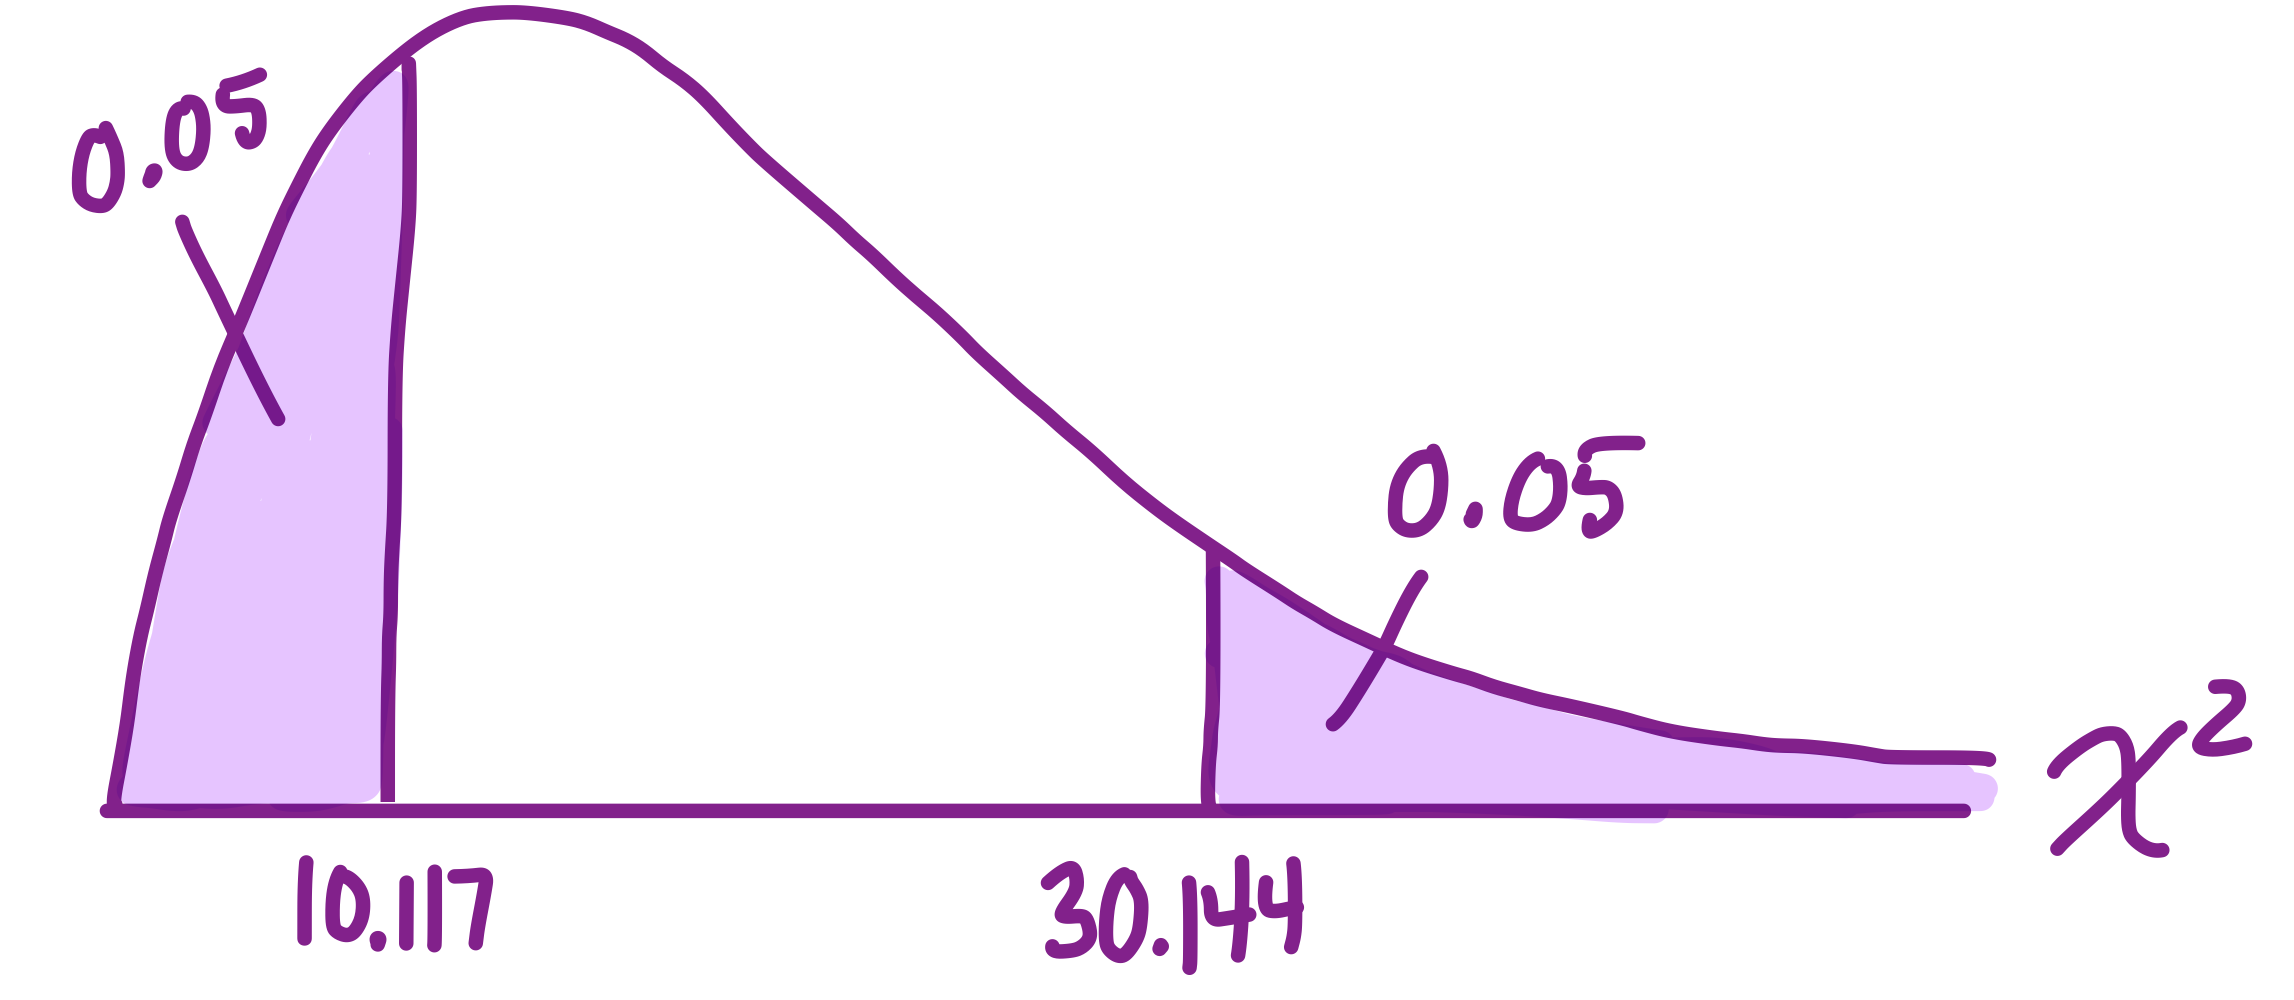
\includegraphics[scale=0.09]{STAT_3090_Ch10_ChiSquare.JPEG}
    
    $\alpha=0.10 \Rightarrow \nicefrac{\alpha}{2}=0.05$
	
	$df=20-1=19$
	
	$\chi_{.95,19}^2=10.117$
	
	$\chi_{.05,19}^2=30.144$
	
	RR: $\chi^2<10.117$ or $\chi^2>30.144$
	
	
	\end{multicols}

	\end{solution}	
	
	\question What is your decision about the null hypothesis? Provide support for your decision.
	
	\begin{solution}[\stretch{1}]
	
	\vspace{1mm}
	
	Because $\chi_0^2=30.53>30.144$ (i.e. the test statistic is in the rejection region), we reject $H_0$. 
	
	\vspace{1mm}
	
	\end{solution}
	
%	\newpage 
	
	\question Summarize the results of your test in context.
	
	\begin{solution}[\stretch{1}]
	
	\vspace{1mm}
	
	At the $\alpha=0.10$ level, we have sufficient evidence that...
	\begin{itemize}
	\item the true variance of Ramen sodium levels using the new ingredients is different than 12,100 mg$^2$.
	\item the true standard deviation of Ramen sodium levels using the new ingredients is different than 110 mg.
	\item the true variance / standard deviation of Ramen sodium levels has changed with the new ingredients.
	\end{itemize}
	(Any of the above would be correct.)
	\end{solution}
	
\newpage

\question Suppose that a media research group believes that the average age by which an individual under 25 has seen all 8 Harry Potter films is 14 years old. You want to see if this average is higher for students in your residence hall. You take a random sample of 65 fellow students from your dorm and find that the average age by which they had seen all 8 films is 14.8 years old with a standard deviation of 4.5 years old. Test your hypothesis at the $\alpha=0.01$ level using the \textbf{rejection region} approach.

\vspace{3mm}

\begin{parts}

\part Define the \textbf{parameter} of interest and state the \textbf{hypotheses}.

\begin{solution}[\stretch{1}]

\vspace{3mm}

Let $\mu=$ the true mean age by which students in your dorm have seen all eight Harry Potter films.

\vspace{3mm}

$H_0:\mu=14$

$H_1:\mu>14$

\vspace{3mm}

\end{solution}

\part Verify that the necessary \textbf{assumptions} hold.

\begin{solution}[\stretch{1}]

\vspace{3mm}

(1) The sample must be randomly selected from the target population --- it is stated in the problem that you took a random sample of 65 students from those in your dorm.

\vspace{3mm}

(2) The sampling distribution of $\overline{X}$ must be approximately normally distributed --- this is true by the Central Limit Theorem because $n=65>30$.

\vspace{3mm}

\end{solution}

\part Conduct your test by finding the \textbf{test statistic} and using the \textbf{rejection region} approach.

\begin{solution}[\stretch{1}]

\vspace{3mm}

\underline{Test Statistic}: $t_0=\displaystyle\frac{\overline{x}-\mu_0}{\nicefrac{s}{\sqrt{n}}}=\frac{14.8-14}{\nicefrac{4.5}{\sqrt{65}}}=1.43$

\vspace{3mm}

\underline{Critical Value}: $H_1$ indicates a \textit{right}-tailed test, so choose the $t$ critical value with an area of $\alpha=0.01$ to the \textit{right} and $df=65-1=64$.

\vspace{3mm}

$t_{.01,64}=\text{invT}(1-.01,64)=2.386$ \hspace{55mm} Rejection Region: $T>2.386$

\vspace{3mm}

\begin{tikzpicture}
        \def\normaltwo{\x,{2*1/exp(((\x-3)^2)/2)}}
        \def\y{5}
        \def\mu{3}
        \def\fy{2*1/exp(((\y-3)^2)/2)}
        \fill [fill=purp!30] (\y,-.1) -- plot[domain=\y:6.5] (\normaltwo) -- (6.5,-.1) -- cycle;
        \draw[domain=-.5:6.5,samples=100] plot (\normaltwo) node[right] {};
        \draw[dashed] ({\y},{\fy}) -- ({\y},-.15) node[below] {\small{$t_{.01,64}$}};
        \node at ({\y},-.8) {\small{$2.386$}};
        \draw[] ({\mu},{0}) -- ({\mu},-.1) node[below] {\small{$0$}};
        \draw[-] (-.7,-.1) -- (6.7,-.1) node[right] {};
        \node[] at (7.0,-.1) {$T$};
        \node[] at (5.5,1) {$0.01$};
        \draw[-] (5.5,0.8) -- (5.2,.1);
        \node at (3,1) {$0.99$};
  \end{tikzpicture}

\vspace{3mm}

\end{solution}

\part What is your decision about the null hypothesis $H_0$? Justify your answer with the appropriate \textbf{support} from your test results.

\begin{solution}[\stretch{1}]

\vspace{3mm}

We do not reject $H_0$ because the test statistic $t_0$ is not in the rejection region ($1.43<2.386$).

\vspace{3mm}

\end{solution} 

\part \textbf{Summarize} the results of your test in context.

\begin{solution}[\stretch{1}]

\vspace{3mm}

At the $\alpha=0.01$ significance level, we do not have sufficient evidence that the true mean age by which students in the dorm have seen all eight Harry Potter Films is higher than 14 years old (i.e.\ higher than the mean age for all individuals under 25 years old). 

\vspace{3mm}

\end{solution} 

\end{parts}

\newpage

\question Tony Stark is developing a new model of the Iron Man suit. His previous suit model uses an average of 222.4 kilowatts (kW), and he wishes to see if his new model is more efficient (in other words, if the mean energy consumption in kW is less than the previous model). He takes a sample of five randomly selected suits made under the new model and finds that the mean energy consumption is 210.2 kW with a standard deviation of 9.9 kW. He knows that the energy consumption for a given suit follows a normal distribution based on his previous tests. Test Tony's hypothesis at the $\alpha=0.05$ significance level using the \textbf{p-value} approach.

\vspace{3mm}

\begin{parts}

\part Define the \textbf{parameter} of interest and state the \textbf{hypotheses}.

\begin{solution}[\stretch{1}]

\vspace{3mm}

Let $\mu=$ true mean energy consumption in kW for the new Iron Man suit model.

\vspace{3mm}

$H_0:\mu=222.4$ kW

$H_1:\mu<222.4$ kW

\vspace{3mm}

\end{solution} 

\part State and verify the necessary \textbf{assumptions}.

\begin{solution}[\stretch{1}]

\vspace{3mm}

(1) Must have a random sample selected from the population --- the problem states that the five suits were randomly selected.

\vspace{3mm}

(2) $\overline{X}$ must be approximately normally distributed --- this is true since we know that the population energy consumption is normally distributed (stated).

\vspace{3mm}

\end{solution} 

\part Conduct your test by finding the \textbf{test statistic} and using the \textbf{p-value} approach.

\begin{solution}[\stretch{1}]

\vspace{3mm}

\underline{Test Statistic}: $t_0=\displaystyle\frac{\overline{x}-\mu_0}{\nicefrac{s}{\sqrt{n}}}=\frac{210.2-222.4}{\nicefrac{9.9}{\sqrt{5}}}=-2.76$

\vspace{3mm}

\underline{P-Value}: $p$-value $=P(T<-2.76)=\text{tcdf}(-\text{1\sc{e}99},-2.76,4)=0.0254$

\vspace{3mm}

\begin{tikzpicture}
        \def\normaltwo{\x,{2*1/exp(((\x-3)^2)/2)}}
        \def\y{1.2}
        \def\mu{3}
        \def\fy{2*1/exp(((\y-3)^2)/2)}
        \fill [fill=purp!30] (-.5,-.1) -- plot[domain=-.5:\y] (\normaltwo) -- (\y,-.1) -- cycle;
        \draw[domain=-.5:6.5,samples=100] plot (\normaltwo) node[right] {};
        \draw[dashed] ({\y},{\fy}) -- ({\y},-.15) node[below] {\small{$-2.76$}};
        \draw[] ({\mu},{0}) -- ({\mu},-.1) node[below] {\small{$0$}};
        \draw[-] (-.7,-.1) -- (6.7,-.1) node[right] {};
        \node[] at (7.0,-.1) {$T$};
        \node[] at (0.7,1) {$0.0254$};
        \draw[-] (0.7,0.8) -- (0.9,.1);
 \end{tikzpicture}

\vspace{3mm}

\end{solution} 

\part Provide \textbf{support} for your decision regarding the null hypothesis.

\begin{solution}[\stretch{1}]

\vspace{3mm}

We reject $H_0$ because the $p$-value is less than the significance level $\alpha$ ($0.0254<0.05$).

\vspace{3mm}

\end{solution}

\part \textbf{Summarize} the results of your test in context.

\begin{solution}[\stretch{1}]

\vspace{3mm}

At the $\alpha=0.05$ significance level, we have sufficient evidence that the true mean energy consumption for the new Iron Man suit is less than 222.4 kW (i.e.\ that the mean energy consumption for the new suit is lower than the previous model). 

\vspace{3mm}

\end{solution}

\end{parts}

\newpage

\question Dunder Mifflin recently expanded its supply to include not just paper, but also copiers. David Wallace, the chief financial officer, claims that the expansion is a smashing success, with the copier production process producing defective parts only 0.7\% of the time.
    
    \vspace{3mm}
        
    Michael Scott is not superstitious\dots but he is a little stitious. He believes that David Wallace's claim is incorrect. He randomly selects 750 copier parts and finds 12 that are defective. Do these data provide evidence at the 10\% level that the proportion of defective copier parts is \textbf{not} 0.7\%?

\vspace{3mm}

\begin{parts}

\part Define the \textbf{parameter} of interest and state the \textbf{hypotheses}.

\begin{solution}[\stretch{1}]

\vspace{3mm}

Let $p=$ the true proportion of defective copier parts at Dunder Mifflin.

\vspace{3mm}

$H_0: p = 0.007$

$H_1: p \neq 0.007$

\vspace{3mm}

\end{solution}

\part Verify that the necessary \textbf{assumptions} hold.

\begin{solution}[\stretch{1}]

\vspace{3mm}

(1) Random sample --- stated that Michael randomly selects the copier parts.

\vspace{3mm}

(2) $\hat{p}$ must be approx.\ normal --- true because $np_0=750(0.007)\geq 5$ and $n(1-p_0)=750(0.993)\geq 5$.

\vspace{3mm}

\end{solution}

\part Calculate the appropriate \textbf{test} statistic. Show your work.

\begin{solution}[\stretch{1}]

\vspace{3mm}

$\displaystyle z_0=\frac{\hat{p}-p_0}{\sqrt{\frac{p_0(1-p_0)}{n}}}=\frac{\frac{12}{750}-0.007}{\sqrt{\frac{0.007(1-0.007)}{750}}} = 2.96$

\vspace{3mm}

\end{solution}

\part Find the \textbf{rejection region}. Include a sketch showing where your test statistic falls relative to the RR.

\begin{solution}[\stretch{1}]

\vspace{3mm}

$\alpha=0.1 \; \Rightarrow$ \underline{Critical Value}:  $z_{\nicefrac{\alpha}{2}}=z_{.05}=1.64$ \hspace{30mm} RR: $Z>1.64$ or $Z<-1.64$

\vspace{3mm}

\begin{tikzpicture}
        \def\normaltwo{\x,{2*1/exp(((\x-3)^2)/2)}}
        \def\y{1.5}
        \def\mu{3}
        \def\z{4.5}
        \def\fy{2*1/exp(((\y-3)^2)/2)}
        \def\fz{2*1/exp(((\z-3)^2)/2)}
        \fill [fill=purp!30] (-.5,-.1) -- plot[domain=-.5:\y] (\normaltwo) -- (\y,-.1) -- cycle;
        \fill [fill=purp!30] (\z,-.1) -- plot[domain=\z:6.5] (\normaltwo) -- (6.5,-.1) -- cycle;

        \draw[domain=-.5:6.5,samples=100] plot (\normaltwo) node[right] {};
        \draw[dashed] ({\y},{\fy}) -- ({\y},-.15) node[below] {\small{$-1.64$}};
        \draw[dashed] ({\z},{\fz}) -- ({\z},-.15) node[below] {\small{$1.64$}};

        \draw[] ({\mu},{0}) -- ({\mu},-.1) node[below] {\small{$0$}};
        \draw[-] (-.7,-.1) -- (6.7,-.1) node[right] {};
        \node[] at (7.0,-.1) {$Z$};
        \node[] at (0.7,1) {$0.05$};
        \draw[-] (0.7,0.8) -- (0.9,.1);
        \node[] at (5.3,1) {$0.05$};
        \draw[-] (5.3,0.8) -- (5.1,.1);
        
        \draw[] (5.5,{0}) -- (5.5,-.1) node[below] {\small{$2.96$}};
 \end{tikzpicture}

\vspace{3mm}

\end{solution} 

\part Use the results of the test to provide \textbf{support} for your decision about the null hypothesis.

\begin{solution}[\stretch{1}]

\vspace{3mm}

Because $z_0=2.96>1.64$ ($z_0$ is in the rejection region), we reject $H_0$.

\vspace{3mm}

\end{solution}

\part \textbf{Summarize} the results of your hypothesis test in context.

\begin{solution}[\stretch{1}]

\vspace{3mm}

At the $\alpha=0.1$ significance level, we have sufficient evidence that the true proportion of defective parts at Dunder Mifflin is not 0.7\% (i.e.\ we have sufficient evidence that David Wallace's claim is incorrect). 

\vspace{3mm}

\end{solution} 

\end{parts}

%\newpage 

\question As regional co-manager of Dunder Mifflin, Jim suggests using the $p$-value approach to double check behind Michael. Find the appropriate $p$-value (use appropriate probability notation) and provide support for a decision about $H_0$. Does your conclusion change at all?

\begin{solution}[\stretch{1}]

\vspace{3mm}

$p$-value $=2\times P(Z>2.96)=2\times \text{normalcdf}(2.96,1\text{\sc{e}}99,0,1)=2(0.001538)=0.0031$

\vspace{3mm}

Reject $H_0$ because $p$-value $=0.0031<\alpha=0.1$. The conclusion does not change.

\vspace{3mm}

\end{solution} 


\newpage

\fullwidth{An expensive new type of fertilizer is being tested on a plot of land at Schrute Farms to see whether it increases the amount of beets produced. The mean number of pounds of beets produced on this plot with the old fertilizer is 400 pounds. Dwight believes that the mean yield will increase with the new fertilizer.}

\vspace{4mm}

\question Define the \textbf{target parameter} in this scenario.

\begin{solution}[\stretch{1}]

\vspace{1mm}

$\mu=$ the true mean beet yield (in pounds) of the plot with the new fertilizer

\vspace{1mm}

\end{solution}

\question Determine the \textbf{null and alternative hypotheses} in this problem.

\begin{solution}[\stretch{1}]

\vspace{1mm}

$H_0:\mu=400$ lb

$H_1:\mu>400$ lb

\vspace{1mm}

\end{solution}

\question Is this a left-tailed, right-tailed, or two-tailed test?

\begin{solution}[\stretch{1}]

\vspace{1mm}

Right-tailed

\vspace{1mm}

\end{solution}

\question Describe a \textbf{Type I error} in context of the problem.

\begin{solution}[\stretch{1}]

\vspace{1mm}

Rejecting a true $H_0$: Concluding that the new fertilizer increases yield when it actually does not.

\vspace{1mm}

\end{solution}

\question What might be a \textbf{consequence} of committing a Type I error?

\begin{solution}[\stretch{1}]

\vspace{1mm}

Spending a lot of money on the new fertilizer when it doesn't have an overall positive effect on beet yield.

\vspace{1mm}

\end{solution}

\question Describe a \textbf{Type II error} in context of the problem.

\begin{solution}[\stretch{1}]

\vspace{1mm}

Failing to reject a false $H_0$: Concluding that the new fertilizer does not increase yield when it actually does.

\vspace{1mm}

\end{solution}

\question What might be a \textbf{consequence} of committing a Type II error?

\begin{solution}[\stretch{1}]

\vspace{1mm}

Schrute Farms misses out on potential profit they could have had by increasing their beet yield with the new fertilizer.

\vspace{1mm}

\end{solution}

\question Which of these types of error might we want to minimize? Justify your answer. 

\begin{solution}[\stretch{1}]

\vspace{1mm}

Answers may vary. If a Type II error occurs, Schrute Farms doesn't lose anything tangible, so a Type I error might be more costly and thus have more serious consequences. We would probably want to minimize a Type I error. (You could do this by choosing a smaller significance level $\alpha$.)

\vspace{1mm}

\end{solution}

\end{questions}
%-----------------------------------------------------------------------------%

\end{document}
